\section{Otázky z testů 2023}
\begin{enumerate}
    \item \textbf{Jaká je přenosová rychlost 2B1Q linkvého kodu s periodou $T_s=250 \mu s$}
    \begin{align*}
     M=1/2 * R \\
     M= 1/T_s \\
    1/T_s=1/2 * R \\
    R= 2/T_s \\
    R= 2/250\mu s \\
    R= 8kbit/s
    \end{align*}
    \item \textbf{Jaká je minimální potřebná šířka pasma pro kmitočtové klíčování 505 kHz a 495 kHz, pokud je přenosová rychlost 5 kbit/s}
    \begin{align*}
        f_0=505 kHz \\
        f_1=495 kHz \\
        B= f_0 - f_1 + M  \\
        B= f_0 - f_1 + R  \\
        B= 505-495+5 \\
        B=15 kHz  
    \end{align*}
    Note: M=R - doba symbolu se rovná době prvku
    
    \item \textbf{Jaká je stejnosměrná složka bipolárního kodu RZ, s posloupností 110110 a výškou impulzú -+ 1V a doba symbolu je rovna polovině doby bitu}

    
    \begin{align*}
        A_0 = D*\frac{p*\theta-n*\theta}{T} \\
        A_0 = 1 *\frac{2*0.5-1*0.5}{3} \\
        A_0 = \frac{1}{6}
    \end{align*}

    \item \textbf{Modulace PM s indexem fázové modulace rovným 1.2. Jak se změní fázový zdvih, pokud zvýšíme kmitočet modulačního signálu na dvojnásobek}

    \begin{align*}
        \beta= 1.2 \\
        \varphi = \beta
    \end{align*}
    Odpověd: Nezmění se, fázový zdvih ($\varphi$) se rovná indexu fázové modulace $\beta$ a nezávisí na kmitočtu modulačního signálu.

    \item \textbf{Jaká je šířka pásma, pokud je použito zapojení s Raised-cosine filtrem s indexem $\alpha=0.3$ a bitovou rychlostí 12kbit/s}
    \begin{align*}
        B = (1+ \alpha)*\frac{M}{2} \\
        M= \frac{R}{log_2Q} \\
        M= \frac{R}{log_22} \\
        M=R \\
        B = (1+ 0.3)*\frac{12}{2} \\
        B= 7.8
    \end{align*}
    \item \textbf{Uvažujte šum s Gausovským rozložením a směrodatnou odchylkou 2V. Jaká je efektivní hodnota šumu ? }
    \\
    Odpověd: Efektivní hodnota odpovídá směrodatné odchylce, tedy
    $$\sigma=2$$
    \item  \textbf{Jaký druh modulátoru je na obrázku: MSK, FSK, ASK, QPSK}
    \begin{figure}[h!]
        \centering
        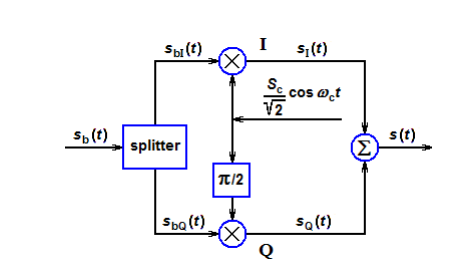
\includegraphics{images/QPSK.png}
        \caption{Modulátor}
        \label{fig:enter-label}
    \end{figure}

    Odpověd: QPSK

    \item \textbf{Jak se u amplitudové modulace nazývá poměr amplitudovéího zdvyhu a aplitudy
  nosného signalu?}
    $$
    m=\frac{\Delta S}{S_c}
    $$
    odpověd: Hloubka modulace


    \item \textbf{4B3T - určit R z M}
    \begin{align*}
    M=\frac{3R}{4}\\
    R=\frac{4M}{3}
    \end{align*}
   
   
    \textbf{\item O-QPSK}
    \begin{figure} [h!]
        \centering
        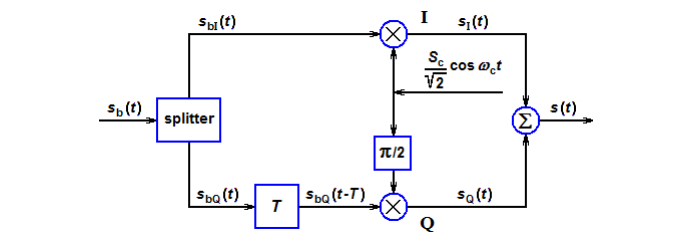
\includegraphics{images/O-QPSK.png}
        \caption{Caption}
        \label{fig:enter-label}
    \end{figure}
    
    \item \textbf{To stejné co otázka 3}

    \item \textbf{Obdobně jako otázka 8 - vzorec na hloubku modulace - co je jmenovatel ?}
     $$
    m=\frac{\Delta S}{S_c}
    $$

    Odpověd: Amplituda nosného signálu

    \item \textbf{Nějaký random odčítání z grafu}
    \begin{verbatim}
         S akou pravdepodobnostou bude hodnota vacsia ako 1? A bolo
         tam rozdelenie pravdepodobnosti
         a distibucna
        funkcia, tak som to len odcital z grafu ze
        1 bola na 0,7 takze odpoved bola 30% moznost.
    \end{verbatim}

    \item  \textbf{Obdobně jako příklad 5, ale vyjádřit $\alpha$}

    \begin{align*}
         B = (1+ \alpha)*\frac{M}{2} \\
     \alpha = \frac{2B}{M}-1
    \end{align*}

    \item 
    Netuším
    \texttt{Dve otazky s frekvenciami ale neviem co presne, ako sa zmeni frekvencny zdvih, a druhe nieco ze zistit 
    dve frekvencne pasma.}

    \item \textbf{FFSK - zjistit přenosovou rychlost}
    \begin{align*}
        f_0=100.325 \\
        f_1= 100.675 \\
        \Delta f = R/4\\
       \Delta f = (f1 - f0) / 2\\
       (f1 - f0) / 2 = R/4\\
        4(f1 - f0) / 2 = R\\
        2(100.675-100.325)=R \\
        R= 0.7Mbit/s
    \end{align*}
    

    \item \textbf{Bipolární signál, D=+- 0.75, P(0)=P(1),  šum s výkonem 0.09W, určit $P_e$}

    Rozhodovací úroveň je tedy optimální, můžu použít jednodušší vzorec
    \begin{align*}
        D_0=-0.75 \\
        D_1=0.75 \\
        P_s = 0.09 => \sigma=\sqrt{0.09}=0.3V \\
        P_e = F_0(\frac{D_0-D_1}{2*\sigma}) \\
        P_e= F_0(-2.5) \\
        P_e= 6.21*10^{-3}
    \end{align*}
    
    \item \textbf{Máme periodický unipolární signál 110110, 1 je vyjadřena pomocí D=-3V, urči stejnosměrnou sloužku.}

    Pokud by byl RZ
\begin{align*}
     A_0 = D*\frac{\theta}{T} \\
        A_0 = -3 *\frac{0.5}{3} \\
        A_0 = -\frac{1}{2}V \\
\end{align*}

\break

\item \textbf{Hlas v pasmu 300 Hz az 3000 Hz v SSB, celková šířka pasma?}
Dle tabulky pro SSB
$$B=f_{max}$$

Odpověď 3kHz

\item \textbf{Signál DSB-SC je součást tzv. stereofonního multiplexního signálu. Horzní mezní kmitočet je 53kHz, dolní 23 kHz. Jaký je horní mezní kmitočet modulačního signálu?}
\begin{align*}
    F_{max}=B/2=\frac{53*10^{-3}-23*10^{-3}}{2} = 15kHz
\end{align*}

\item \textbf{Obrázek pi/4 QPSK}

Note: předpokládám že myslel pi/4 DQPSK

\begin{figure}[h!]
    \centering
    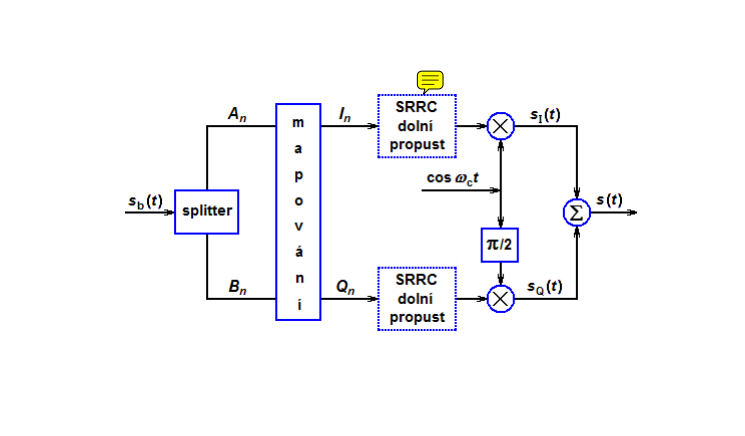
\includegraphics{images/pi.png}
    \caption{pi/4 DQPSK}
    \label{fig:enter-label}
\end{figure}

\item \textbf{Výpočet celkového výkonu, výpočet stejnosměrné složky, minimální šířka pasma}.

 u AM

\begin{align*}
    P_{AM} = P_c + 2P_s \\
    P_c = \frac{S_c^2}{2R}\\
    P_s = \frac{m^2}{4}*\frac{S_c^2}{2R} \\
    B_{min}=2*\Omega
\end{align*}

u FM 
\begin{align*}
    P_{FM}= \frac{S_c^2}{2R}
\end{align*}
šířka pásma dle Carsonových odhadů
\begin{figure}[h!]
    \centering
    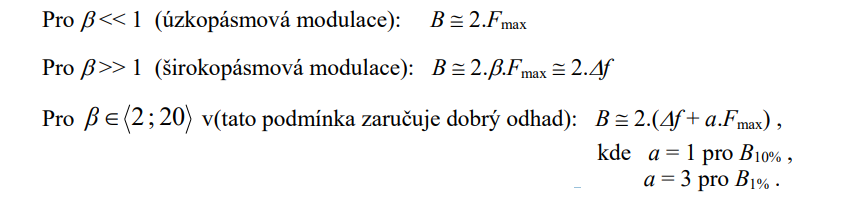
\includegraphics[scale=0.76]{images/Carson.png}
    \caption{Carsonovy odhady}
    \label{fig:enter-label}
\end{figure}
\end{enumerate}
\clearpage
\section{Random otázky z fektušky}
\begin{enumerate}
    \item \textbf{XQAM modulace- výpočet modulační rychlosti}
    
    X vyjadřuje počet stavů tedy Q, platí
    $$
    M=\frac{R}{log_2Q}
    $$
    \item \textbf{Jak se změní výkon kmitočtové modulovaného signálu změnou amiplitudy nosné vlny}
    
    Platí $P_{FM}=\frac{S_c^2}{2R}$, tedy 2x větší $S_c$ = 4x větší $P_{FM}$ atp. 
    \item \textbf{Které z těchto signálů nepatří mezi medolace s harmonickou vlnou}
    \begin{enumerate}
        \item AM
        \item FM
        \item PM
        \item \textbf{PAM} = diskrétní
        \item QAM
        \item QPSK
        \item \textbf{PPM} = diskrétní
    \end{enumerate}
    \item \textbf{Rozpoznat AMI, 4B3T kody}

    Ami- 0 vyjádřena nulovou úrovní, 1 impulzem se střídající se +- polaritou
    4B3T- 4 bitové posloupnosti, "3" urovně v posloupnosti.
    \item  \textbf{Blok na vstupu přijámače, kompenzuje lineární zkreslení signálu}
\begin{enumerate}
    \item AA filitr
    \item deskrambler
    \item Diferenční koder
    \item  \textbf{Ekvalizér}
    \item Expandor
    \item Integrátor
    \item Kompresor
    \item Raised cosine filtr
    \item  Matched filtr
\end{enumerate}
    \item \textbf{Jak velkou bitovou rychlostí přenáší data signál GMSK, jestliže použitý Gaussovský tvarovací 
    filtr má parametr BT = 0,4 a 3decibelová šířka pásma tohoto filtru je 100 kHz}
    \begin{align*}
        BT=0.4 \\
        B= 100 kHz\\
        T_b = ? \\
        R= ? \\
        T_b=\frac{BT}{B}=\frac{0.4}{100*10^3}=4*10^{-6}\\
    R=\frac{1}{T_b}=250 kbit/s
    \end{align*}
    \item  \textbf{Periodicky se opakující posloupnost bitů …1001010010… je vysílána bipolárním impulzovým signálem s napěťovými úrovněmi ±5 V bez návratů k nulové úrovni (NRZ), přičemž bit 1 je reprezentován kladnou úrovní a bit 0 zápornou úrovní napětí. Jaká je velikost stejnosměrné složky tohoto vysílaného signálu?}
    \begin{align*}
         A_0 = D*\frac{p*\theta-n*\theta}{T} \\
         A_0=5*\frac{2*1-3*1}{5} \\
         A_0= -1V
    \end{align*}
    \item J\textbf{aká musí být minimální výška kvantovacího kroku modulace delta (DM), aby nedošlo ke 
    zkreslení přenášeného signálu přetížením kodéru, jestliže chceme touto modulací přenášet 
    signál s maximální strmostí 300 V/s přenosovým kanálem s přenosovou kapacitou 12 kbit/s?}

????
    \begin{align*}
        \Delta=? \\
        strmost = 300 V/s
    \end{align*}
    \item \textbf{Stejnosměrná složka ze spektra}
    \begin{align*}
        C_1=2*A_0*|sinc(\frac{\theta}{2}*k*\omega)| \\
        C_1=4.8|sinc(\frac{\theta}{2}*\frac{2\pi}{4\theta})\\
        C1=4.8|sinc(pi/4)\\
        C_1=4.32
    \end{align*}
    \item \textbf{Stejnosměrná složka ze spektra pro periodický signál}
    \begin{align*} 
        C_1=2*A_0*|sinc(\frac{\theta}{2}*k*\omega)| \\
        C_1=4|sinc(\frac{\theta}{2}*\frac{2\pi}{\frac{5\theta}{2}})\\
        C1=4|sinc(pi/2.5)\\
        C_1=3.03
    \end{align*}
    \item Jaký je horní mezní kmitočet modulačního signálu, jestliže spektrum výsledného amplitudového sinálu s oběma postraními pásmy - DSB- leží v pásmu od 89 do 98 kHz
    \begin{align*}
        f_h=\frac{B}{2}=\frac{98-89}{2}= 4,5 kHz
    \end{align*}
    \item Kolik kvantovacích úrovní má 10 bitový A-D převodník 
    \begin{enumerate}
        \item 2
        \item 9
        \item 10
        \item 100
        \item 256
        \item \textbf{1024}
    \end{enumerate}
    $Q=2^N=1024$
     \item \textbf{Jaká je modulační rychlost kmitočtově klíčovaného signálu s minimálním zdvihem (\textbf{MSK}), 
    jehož signálové prvky mají kmitočty 55,02 kHz a 54,98 kHz?}
    \begin{align*}
    M=R\\
    R=4\Delta f \\
    M=4(54.98-55.02)= \textbf{80}
    \end{align*}
    \item  \textbf{K přenosu dat v přeloženém pásmu rychlostí 15 kBd je použito dvoustavové amplitudové 
klíčování. Jaká je minimální šířka pásma přenosového kanálu?}

    Pro dvoustavové amplitudové klíčování platí $B_{min}=M$, tedy B=\textbf{15kHz}
    \item \textbf{
    Jakou rychlostí přenáší data modulace MSK (Minimum-Shift Keying), jestliže kmitočet nosné 
je 250 MHz a kmitočtový zdvih je 62,5 kHz}

\begin{align*}
    R=1/T \\
    \Delta f= \frac{1}{4T}\\
    T = \frac{1}{4f}=\frac{1}{4*625*10^3}=4*10^{-6} \\
    R=1/T=1/4*10^{-6}=250kbit/s
\end{align*}

    \item Uvažujte fázovou modulaci s indexem$\beta$ = 1,2 rad. Jaký bude mít tato modulace index $\beta$, 
jestliže se úhlový kmitočet harmonického modulačního signálu dvojnásobně zvýší?

    $\beta = \Delta\phi$ - vlivem úhlového kmitočnu se nezmění,
    
    \item Kmitočtová modulace s indexem 6,5 má amplitudu nosné vlny 5 V a kmitočet nosné vlny 910 kHz. Harmonický modulační signál je $cos(8*10^3*\pi*t)$. Jaká je hodnota kmitočtové zdvihu
    \begin{align*}
        \beta=\frac{\Delta}{F} \\
        F= 8*10^3/2 \textrm{ asi?}\\
        \Delta=6.5*4*10^3= 26kHz
    \end{align*}
    \item \textbf{Kmitočtová modulace s indexem 2,5 má kmitočet nosné vlny 900 kHz, amplitudu nosné vlny 
5 V a kmitočtový zdvih 55 kHz. Modulační signál je harmonický. Jaký je kmitočet modulačního 
signálu?}   
 \begin{align*}
     \beta=2.5 \\
     \Delta=55 \\
     F=\Delta/\beta \\
     F=55/2.5=22
 \end{align*}
 
    \item Jak se změní celková kmitočtová šířka pásma amplitudově modulovaného signálu s oběma 
postranními pásmy (DSB), jestliže se maximální kmitočet modulačního signálu zdvojnásobí a 
ostatní parametry modulace zůstanou stejné?

    $B=2Fmax$ - zvětší se dvakrát
    \item modulovaný signál je popsá. rovnicí
     
     \begin{align*}
s(t\lbrack S_c+\Delta S*f(t)]*cos(\omega_ct+\varphi_c)
     \end{align*} kde f(t) je 
normovaný modulační signá.l O jaká druh modulace jde ?

     \textbf{AM}
    \item Klíčovaný signál je popsán rovnicí
    $$s(t)=g(t)*S_c*cos(\omega_ct)$$, kde g(t) je obelníkový klíčovací signál o hodnotách +- 1. O jaký druh klíčování se jedná.

    \textbf{BPSK}
    \item Jak se nazývá funkční blok, používaný v kombinaci s rovnoměrným kvantizátorem například 
při digitalizaci řečového signálu, jehož účelem je docílit konstantního poměru výkonu signálu 
k výkonu kvantovacího šumu (SQNR) v celém rozsahu A/D převodníku?

\textbf{Kompresor}

    \item Jaký minimální kmitočtový zdvih musí mít modulace MSK (Minimum Shift Keying) pro přenos 
dat rychlostí 9,6 kbit/s
\begin{align*}
    \Delta=? \\
    \Delta=1/4T_b\\
    R=1/T_b \\
    \Delta=R/4=2.6kHz
\end{align*}
    \item \textbf{Bipolárním signálem RZ o napěťových úrovních +5 V a –5 V je přenášena periodická datová 
posloupnost …110110110… Doba trvání impulzu je poloviční oproti době trvání bitu, která je 
Tb = 250 $\mu$s. Určete stejnosměrnou složku signálu a modulační rychlost}
\begin{align*}
    A_0=5*\frac{2*\theta-\theta}{T}\\
     A_0=\frac{5}{6}\\
      A_0=0.833 \\
      \\
      M=1/\theta=\frac{1}{\theta}=1/125*10^-6\\
      M=8kBd
\end{align*}
    \item \textbf{Jaká bude šířka pásma B amplitudově modulovaného signálu s jedním postranním pásmem a 
nosnou (SSB), jestliže dolní mezní kmitočet modulačního signálu fd = 10 Hz, horní mezní 
kmitočet modulačního signálu fh = 15 kHz a kmitočet nosné fc = 100 kHz.}

Pro SSB platí $B=Fmax$ tedy B=15kHz

    \item \textbf{Jaká je modulační rychlost systému 32QAM (tj. modulační rychlost na výstupu modulátoru), 
jestliže na vstup modulátoru přivádíme binární NRZ modulační signál s dobou trvání 
signálového prvku 50 $\mu$s? }
\begin{align*}
    M=1/T_s\\
    1/50*10^{-6} \\
    M=20 kBd
\end{align*}
\item \textbf{Jaká musí být minimální výška kvantovacího kroku modulace delta (DM), aby nedošlo ke 
zkreslení přenášeného signálu přetížením kodéru, jestliže chceme touto modulací přenášet 
signál s maximální strmostí 300 V/s přenosovým kanálem s přenosovou kapacitou 12 kbit/s?}
\begin{align*}
    A*\Omega=300V/s \\
    R=12*10^3 \\
    A*\Omega=\frac{\Delta}{T_s}\\
    R=\frac{1}{T_s} \\
    T_s=\frac{1}{R} \\
    T_s=\frac{1}{12*10^3} \\
    300=\frac{\Delta}{\frac{1}{12*10^3}}\\
    \Delta=\frac{300}{12*10^3}\\
    \Delta=0.025 V
\end{align*}
\item \textbf{Uvažujte osmibitovou PCM, maximální kmitočet vstupního signálu je Fmax = 3,4 kHz, 
frekvence vzorkování fv = 48 kHz, rozsah vstupního signálu je od –5 V do +5 V. Kolik bitů musí 
mít DPCM, aby výsledné zkreslení kvantovacím šumem bylo přinejmenším stejné jako 
v případě PCM?}

\begin{align*}
\Delta_{max}=2*\mathrm{VOLTY}sin(2\pi*F_{max}*T_s) \\
T_s=1/48=2.5*10^{-6} \\
    \Delta_{max}=2*5sin(2\pi*3.4*10^3*2.5*10^{-6})=2.33\\
      \Delta_{PCM}=\frac{FS}{2^n}=\frac{10}{2^8}=0.039 \\
    \Delta_{PCM}=\Delta_{DPCM} \\
    0.039=\frac{2\Delta_{max}}{2^n}\\
   N=log_2(\frac{4.66}{0.039})=6.9\Tilde{=}7\mathrm{bitu}
\end{align*}

\end{enumerate}

\section{Schémata modulátorů, klíčování etc. - basic vzorce}
\begin{enumerate}
    \item \textbf{RANDOM USEFUL VZORCE}
    \begin{enumerate}
        \item Stejnosměrná složka
        \begin{enumerate}
            \item Unipolar$$A_0=D*\frac{\theta}{T}$$
            \item Bipolar$$A_0=D\frac{p*\theta-n*\theta}{T}$$\footnote{$\theta$= doba trvání jednoho impulzu - např u bipolar 0.5, většinou v zadání. T= perioda- po kolika bitech se posloupnost opakuje}
        \end{enumerate}
        \item Chybovost $P_e=F_0(\frac{D_0-D_1}{2\sigma})$
        \item Amplituda k-te harmonické složky$$2A_0sinc|\frac{\theta}{2}*\frac{2\pi}{T_0}|$$
    \end{enumerate}
    \item \textbf{AM }
        \begin{enumerate}
            \item Modulovaný signál:
            $$S_c[1+m*f(t)]cos(\omega_ct
            $$, kde f(t) je normovaný modulační signál, m je hloubka modulace
            \item $m=\frac{\Delta S}{S_c}$
            \item $B=2\Omega$
            \item $S_s=1/2\Delta S$
            \item $P_{AM}=P_c+2P_s$
            \item $P_c=\frac{S_c^2}{2R}$
            \item $P_s=\frac{m^2*S_c^2}{8R}$
            \item SSB - B= $\Omega_{max}$ a $P=P_c+P_s$
            \item SSB-PSC B= $\Omega_{max}$ a $P=a^2P_c+P_s$
            \item SSB-SC B=$\Omega_{max}-\Omega_min$ a $P=P_s$
            \item DSB-SC B=B=$2\Omega_max$ a $P=2P_s$
        \end{enumerate}
    \item FM
    \begin{enumerate}
        \item Modulovaný signál: $$
        S_ccos[\phi (t)+\varphi_c]
        $$,kde $\phi (t)$ je okamžitá fáze.
        \item $B=2*(\Delta f + F_{max}$
        \item $\frac{\Delta f}{F}$
    \end{enumerate}
    \item PM
    \begin{enumerate}
        \item  Modulovaný signál: $$
    s(t)=S_ccos[\omega_ct+\varphi_c+\Delta\varpi f(t)]$$, kde f(t) je normovaný modulační signál
        \item 
    \end{enumerate}
\textbf{    \item ASK}
    \begin{enumerate}
         \item Lze jej popsat jako:
    $$s(t)=s_c(t)*g(t)$$,kde $s_c$ je harmonická nosná vlna a $g(t)$ je obdélníkový klíčovací signál = 0-1
    \item\begin{figure}[h!]
        \centering
        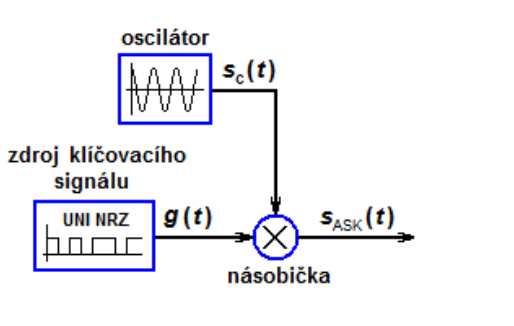
\includegraphics[scale=0.5]{images/ask.png}
        \caption{ASK}
        \label{fig:enter-label}
    \end{figure}
    \item $B_{min}=2F$
    \item $R=M$
    \item $M=\frac{1}{2T_s}$
    \item Kmitočet klíčovacího signálu: $F=1/2T_s$.\footnote{$T_s$=doba trv ání symbolu}

    \end{enumerate}
    \item \textbf{FSK}
    \begin{enumerate}
        \item 1 a 0 reprezentovány harmonickým signálem s kmitočty $f_1$ a $f_0$
            \item $B_{min}=|f_0-f_1|+2F$
        \item $R=M$
    \end{enumerate}
    \item \textbf{BPSK}
    \begin{enumerate}
        \item Lze jej popsat jako $$s(t)=s_c(t)*g(t)$$, kde $s_c$ je harmonicky signal a $g(t)$ je obdelníkový modulační signál 1 a -1
        \item \begin{figure}[h!]
            \centering
            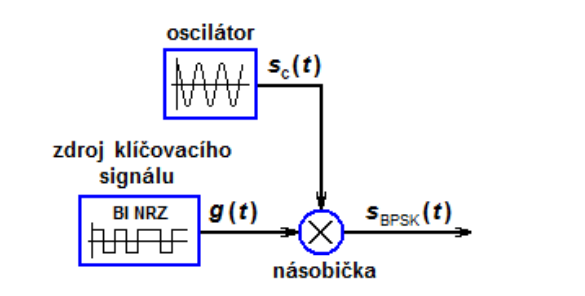
\includegraphics[scale=0.5]{images/BPSK.png}
            \caption{BPSK}
            \label{fig:enter-label}
        \end{figure}
        \item $F_s=\frac{1}{2T_s}$
        \item $M=\frac{1}{T_s}$
        \item $B_{min}=2F=M$
        \item $R=M=B$ asi?
    \end{enumerate}
   \item \textbf{MSK}
   \begin{enumerate}
       \item Zvláštní případ FSK, neobsahuje fázové skoky.
       \item Kmitočtový zdvih $\Delta f= R/4=1/4T$\footnote{T=doba trvani bitu}
       \item hodnota $\Delta f$ je nejmenší hodnota kde lze docílit koherentní demodulace
       \item \begin{figure}[h!]
           \centering
           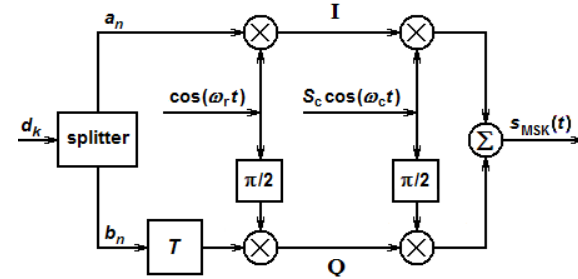
\includegraphics[scale=0.5]{images/MSK.png}
           \caption{MSK}
           \label{fig:enter-label}
       \end{figure}
   \end{enumerate}
   \item \textbf{FFSK}
   \begin{enumerate}
       \item Zvláštní případ FSK, nemá fázové skoky
       \item Popsán rovnicí $$s(t)=S_ccos(\omega_ct+d_k\omega_rt+\varphi_k$$, kde $\varphi_k v intervalu 0 rad - \pi rad$
        \item Kmitočtový zdvih $\Delta f= R/4=1/4T$
       \item \begin{figure}[h!]
           \centering
           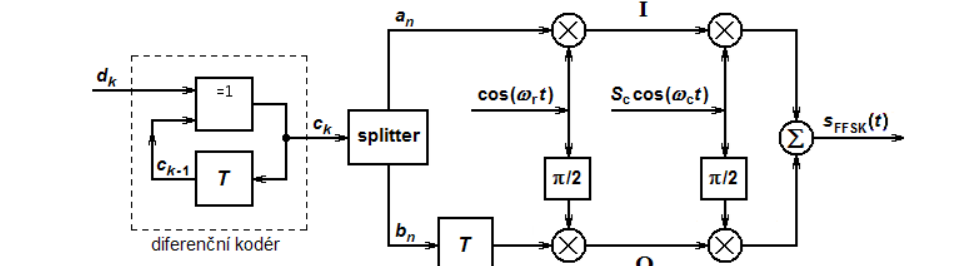
\includegraphics[scale=0.5]{images/FFSK.png}
           \caption{FFSK}
           \label{fig:enter-label}
       \end{figure}
   \end{enumerate}
    \item \textbf{GMSK}
    \begin{enumerate}
        \item varianta FSK, používá gaussovský tvarovací filtr
        \item $B=\frac{BT}{T}$
        \item $T=\frac{1}{R}$
        \item $\Delta f=\frac{1}{4T}$
        \item Spek. účinnost $\frac{R}{B_{ch}}$
        \item \begin{figure}[h!]
            \centering
         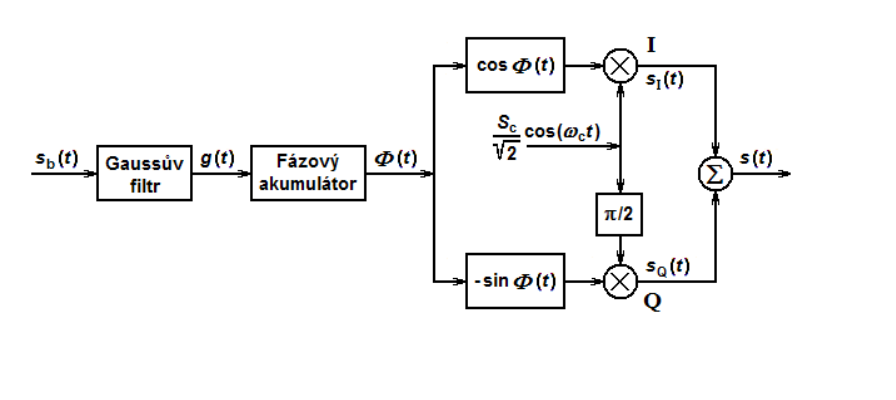
\includegraphics[scale=0.5]{images/GMSK.png}
            \caption{GMSK}
            \label{fig:enter-label}
        \end{figure}
    \end{enumerate}
    \item \textbf{QPSK}
    \begin{enumerate}
        \item \begin{figure}[h!]
            \centering
            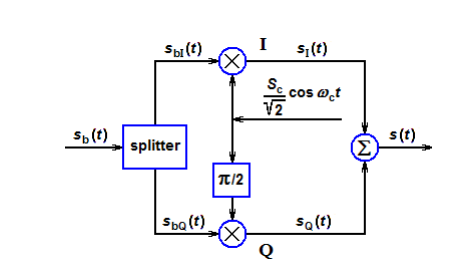
\includegraphics{images/QPSK.png}
            \caption{QPSK}
            \label{fig:enter-label}
        \end{figure}
        \item 4 stavy
        \item \begin{figure}[h!]
            \centering
            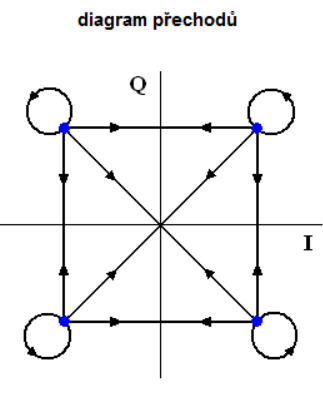
\includegraphics[scale=0.5]{images/QPSKDIAG.png}
            \caption{QPSK diagram prechodu}
            \label{fig:enter-label}
        \end{figure}
    \end{enumerate}
    \clearpage
    \item O-QPSK
    \begin{itemize}
        \item \begin{figure}[h!]
            \centering
            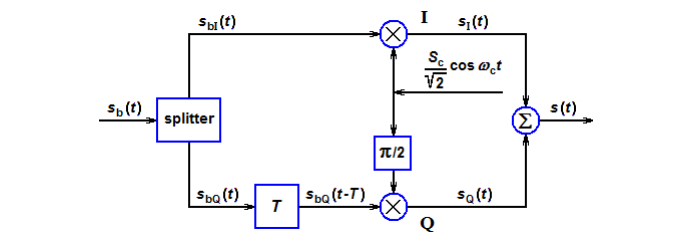
\includegraphics[scale=0.5]{images/O-QPSK.png}
            \caption{O-QPSK}
            \label{fig:enter-label}
        \end{figure}
    \end{itemize}
    \item \textbf{$\pi/4 $DQPSK}
    \begin{enumerate}
        \item \begin{figure}[h!]
            \centering
            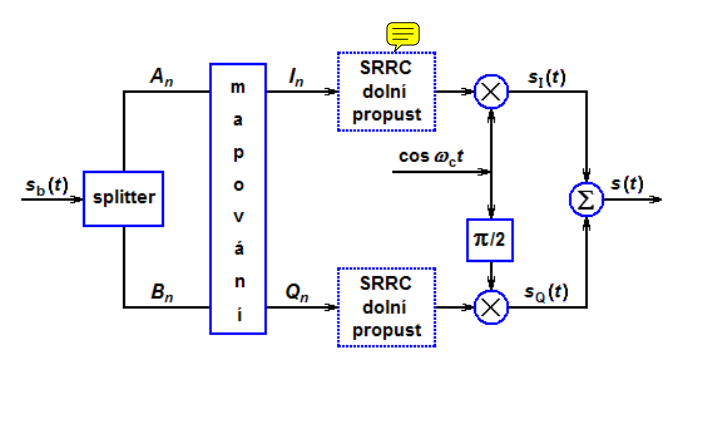
\includegraphics[scale=0.5]{images/DQPSK.png}
            \caption{DQPSK}
            \label{fig:enter-label}
        \end{figure}
    \end{enumerate}
    \item \textbf{MQAM}
    \begin{enumerate}
        \item  M-stavový (Q) modulátor
        \item \begin{figure}
    \centering
    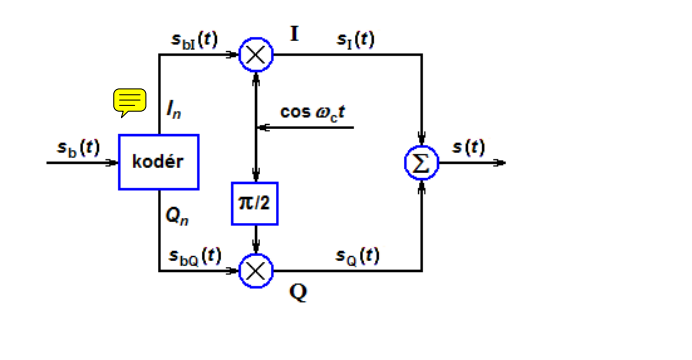
\includegraphics[scale=0.5]{images/MQAM.png}
    \caption{MQAM}
    \label{fig:enter-label}
\end{figure}
    \item  přesnosová rychlost $R=M*log_2Q$
    \item mod. rychlost $M=\frac{1}{T_s}$
     \item počet stavů $Q=2^{\frac{R}{M}}$
     \item úrovně signálu $L_{I,Q}=\sqrt{Q}$\footnote{zaokrouhleno vždy nahoru}
    \end{enumerate}
    \item \textbf{Sample and Hold}
    \begin{enumerate}
        \item šířka impůzu je rovna vzorkovací periodě
        \item Pokles amplitudy demodulovaného signálu $sinc(\pi\frac{F_{max}}{F_s})$
        \begin{figure}[h!]
            \centering
            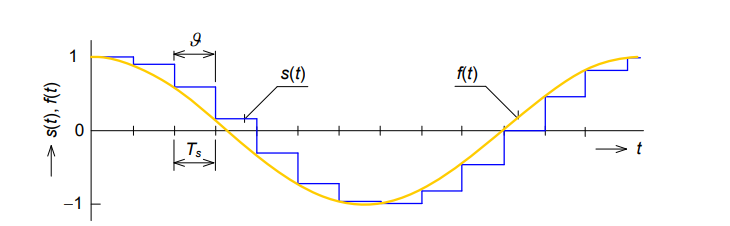
\includegraphics[scale=0.5]{images/SampleHold.png}
            \caption{Caption}
            \label{fig:enter-label}
        \end{figure}
    \end{enumerate}
    \item \textbf{PWM}
    \begin{enumerate}
        \item šířka impulsu se rovná aktuální hodnotě modulačního signálu
        \item note: ty vzorce jsou takové mrdky že nevěřím že tam něco z toho dá
        \item \begin{figure}[h!]
            \centering
            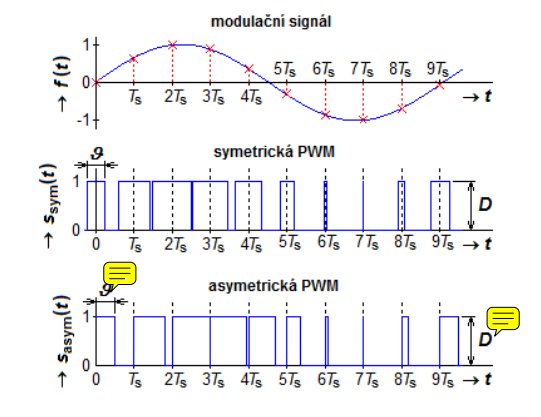
\includegraphics[scale=0.5]{images/PWM.png}
            \caption{Caption}
            \label{fig:enter-label}
        \end{figure}
    \end{enumerate}
    \item \textbf{PPM}
    \begin{enumerate}
        \item Při modulaci PPM je okamžitá hodnota signálu vyjádřena časovou polohu impulzu v daném rámci, šířká odpovídá vzorkovací periodě $T_s$
        \item \begin{figure}[h!]
            \centering
            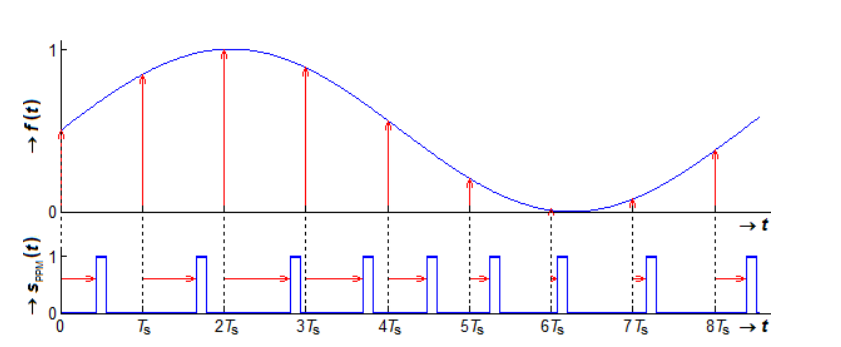
\includegraphics[scale=0.5]{images/PPM.png}
            \caption{PPM}
            \label{fig:enter-label}
        \end{figure}
    \end{enumerate}
    \clearpage
    \item \textbf{PCM}
    \begin{enumerate}
        \item \begin{figure}[h!]
        \centering
        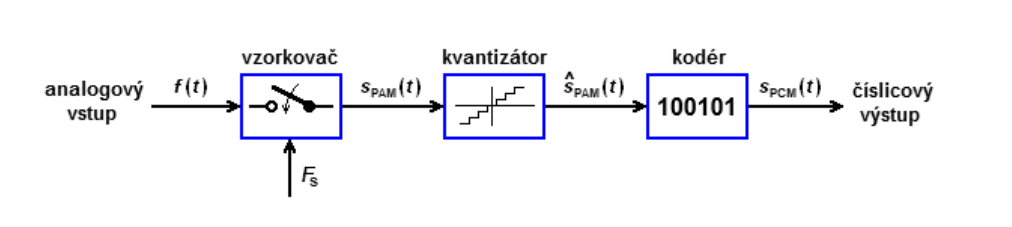
\includegraphics[scale=0.5]{images/pcmdiag.png}
        \caption{PCM}
        \label{fig:enter-label}
        \end{figure}
        \item kvantovací krok $\Delta=\frac{FS}{2^N}$
        \item  FS= rozsah převodníku, N =počet bitů převodníku na vzorek
        \item Dynamický rozsah  $=2^N-1\Tilde{=}2^N$
        \item v DB $DR_{dB}=20log(\frac{FS}{\Delta})$
        \item Střední výkon kvantovacího šumu $P_{sum}=\frac{\Delta^2}{12}$
        \item Střední výkon harm. signálu $P_s=U^2_{ef}=\frac{A^2}{2}$
        \item Odstup signal sum $SQNR=10log(\frac{P_s}{P_{sum}})dB$
        \item Efektivní hodnota kvantovacího šumu $U_{ef_{sum}}=\sqrt{P_{sum}}$
    \item \begin{figure}[h!]
        \centering
        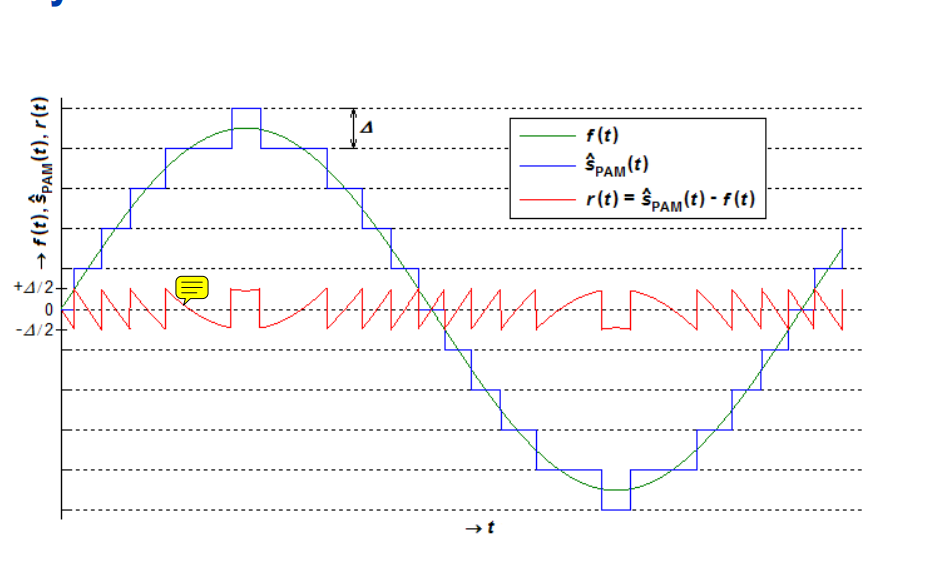
\includegraphics[scale=0.5]{images/pcm.png}
        \caption{Signal v PCM modulatoru}
        \label{fig:enter-label}
    \end{figure}
    \end{enumerate}
    \item \textbf{Delta modulator}
    \begin{enumerate}
        \item Aby nedošlo k přetížení, platí $A*\Omega<\Delta/T_s$
        \item $A*2\pi F_{max}<\Delta*f_s$
        \item $T_s=T_b$
        \item $R=\frac{1}{T_b}$
        \item Strmost=$A*\Omega$
        \item $R=f_s$
\begin{figure}[h!]
        \centering
        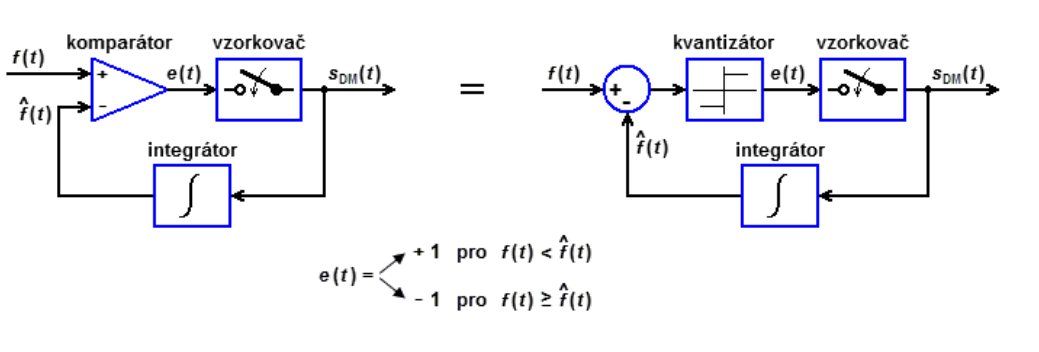
\includegraphics[scale=0.5]{images/delta.png}
        \caption{Delta Modulator}
        \label{fig:enter-label}
    \end{figure}
    \end{enumerate}
    \item\textbf{DPCM}
    \begin{enumerate}
        \item maximalni diference $\Delta_{max}=2*s_{max}*(5*10^6)=2*\mathrm{VOLTY}sin(2\pi*F_{max}*5*T_s)$
        \item$ T_s=1/f_s$
    \end{enumerate}
    \item \textbf{Raised-Cosine filter}
    \item $M=\frac{R}{log_2Q}$
    \item $R=Mlog_2Q$
    \item $B=(1+\alpha)*\frac{M}{2}$
    \item spektral uč. $\frac{R}{B}$
    
\end{enumerate}
